\documentclass[1p]{elsarticle_modified}
%\bibliographystyle{elsarticle-num}

%\usepackage[colorlinks]{hyperref}
%\usepackage{abbrmath_seonhwa} %\Abb, \Ascr, \Acal ,\Abf, \Afrak
\usepackage{amsfonts}
\usepackage{amssymb}
\usepackage{amsmath}
\usepackage{amsthm}
\usepackage{scalefnt}
\usepackage{amsbsy}
\usepackage{kotex}
\usepackage{caption}
\usepackage{subfig}
\usepackage{color}
\usepackage{graphicx}
\usepackage{xcolor} %% white, black, red, green, blue, cyan, magenta, yellow
\usepackage{float}
\usepackage{setspace}
\usepackage{hyperref}

\usepackage{tikz}
\usetikzlibrary{arrows}

\usepackage{multirow}
\usepackage{array} % fixed length table
\usepackage{hhline}

%%%%%%%%%%%%%%%%%%%%%
\makeatletter
\renewcommand*\env@matrix[1][\arraystretch]{%
	\edef\arraystretch{#1}%
	\hskip -\arraycolsep
	\let\@ifnextchar\new@ifnextchar
	\array{*\c@MaxMatrixCols c}}
\makeatother %https://tex.stackexchange.com/questions/14071/how-can-i-increase-the-line-spacing-in-a-matrix
%%%%%%%%%%%%%%%

\usepackage[normalem]{ulem}

\newcommand{\msout}[1]{\ifmmode\text{\sout{\ensuremath{#1}}}\else\sout{#1}\fi}
%SOURCE: \msout is \stkout macro in https://tex.stackexchange.com/questions/20609/strikeout-in-math-mode

\newcommand{\cancel}[1]{
	\ifmmode
	{\color{red}\msout{#1}}
	\else
	{\color{red}\sout{#1}}
	\fi
}

\newcommand{\add}[1]{
	{\color{blue}\uwave{#1}}
}

\newcommand{\replace}[2]{
	\ifmmode
	{\color{red}\msout{#1}}{\color{blue}\uwave{#2}}
	\else
	{\color{red}\sout{#1}}{\color{blue}\uwave{#2}}
	\fi
}

\newcommand{\Sol}{\mathcal{S}} %segment
\newcommand{\D}{D} %diagram
\newcommand{\A}{\mathcal{A}} %arc


%%%%%%%%%%%%%%%%%%%%%%%%%%%%%5 test

\def\sl{\operatorname{\textup{SL}}(2,\Cbb)}
\def\psl{\operatorname{\textup{PSL}}(2,\Cbb)}
\def\quan{\mkern 1mu \triangleright \mkern 1mu}

\theoremstyle{definition}
\newtheorem{thm}{Theorem}[section]
\newtheorem{prop}[thm]{Proposition}
\newtheorem{lem}[thm]{Lemma}
\newtheorem{ques}[thm]{Question}
\newtheorem{cor}[thm]{Corollary}
\newtheorem{defn}[thm]{Definition}
\newtheorem{exam}[thm]{Example}
\newtheorem{rmk}[thm]{Remark}
\newtheorem{alg}[thm]{Algorithm}

\newcommand{\I}{\sqrt{-1}}
\begin{document}

%\begin{frontmatter}
%
%\title{Boundary parabolic representations of knots up to 8 crossings}
%
%%% Group authors per affiliation:
%\author{Yunhi Cho} 
%\address{Department of Mathematics, University of Seoul, Seoul, Korea}
%\ead{yhcho@uos.ac.kr}
%
%
%\author{Seonhwa Kim} %\fnref{s_kim}}
%\address{Center for Geometry and Physics, Institute for Basic Science, Pohang, 37673, Korea}
%\ead{ryeona17@ibs.re.kr}
%
%\author{Hyuk Kim}
%\address{Department of Mathematical Sciences, Seoul National University, Seoul 08826, Korea}
%\ead{hyukkim@snu.ac.kr}
%
%\author{Seokbeom Yoon}
%\address{Department of Mathematical Sciences, Seoul National University, Seoul, 08826,  Korea}
%\ead{sbyoon15@snu.ac.kr}
%
%\begin{abstract}
%We find all boundary parabolic representation of knots up to 8 crossings.
%
%\end{abstract}
%\begin{keyword}
%    \MSC[2010] 57M25 
%\end{keyword}
%
%\end{frontmatter}

%\linenumbers
%\tableofcontents
%
\newcommand\colored[1]{\textcolor{white}{\rule[-0.35ex]{0.8em}{1.4ex}}\kern-0.8em\color{red} #1}%
%\newcommand\colored[1]{\textcolor{white}{ #1}\kern-2.17ex	\textcolor{white}{ #1}\kern-1.81ex	\textcolor{white}{ #1}\kern-2.15ex\color{red}#1	}

{\Large $\underline{12n_{0487}~(K12n_{0487})}$}

\setlength{\tabcolsep}{10pt}
\renewcommand{\arraystretch}{1.6}
\vspace{1cm}\begin{tabular}{m{100pt}>{\centering\arraybackslash}m{274pt}}
\multirow{5}{120pt}{
	\centering
	\includegraphics[width=112pt]{../../../GIT/diagram.site/Diagrams/png/2576_12n_0487.png}\\
\ \ \ A knot diagram\footnotemark}&
\allowdisplaybreaks
\textbf{Linearized knot diagam} \\
\cline{2-2}
 &
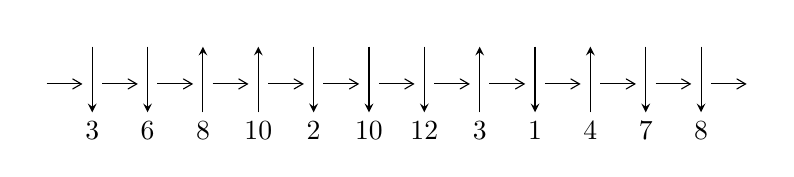
\begin{tikzpicture}[x=20pt, y=17pt]
	% nodes
	\node (C0) at (0, 0) {};
	\node (C1) at (1, 0) {};
	\node (C1U) at (1, +1) {};
	\node (C1D) at (1, -1) {3};

	\node (C2) at (2, 0) {};
	\node (C2U) at (2, +1) {};
	\node (C2D) at (2, -1) {6};

	\node (C3) at (3, 0) {};
	\node (C3U) at (3, +1) {};
	\node (C3D) at (3, -1) {8};

	\node (C4) at (4, 0) {};
	\node (C4U) at (4, +1) {};
	\node (C4D) at (4, -1) {10};

	\node (C5) at (5, 0) {};
	\node (C5U) at (5, +1) {};
	\node (C5D) at (5, -1) {2};

	\node (C6) at (6, 0) {};
	\node (C6U) at (6, +1) {};
	\node (C6D) at (6, -1) {10};

	\node (C7) at (7, 0) {};
	\node (C7U) at (7, +1) {};
	\node (C7D) at (7, -1) {12};

	\node (C8) at (8, 0) {};
	\node (C8U) at (8, +1) {};
	\node (C8D) at (8, -1) {3};

	\node (C9) at (9, 0) {};
	\node (C9U) at (9, +1) {};
	\node (C9D) at (9, -1) {1};

	\node (C10) at (10, 0) {};
	\node (C10U) at (10, +1) {};
	\node (C10D) at (10, -1) {4};

	\node (C11) at (11, 0) {};
	\node (C11U) at (11, +1) {};
	\node (C11D) at (11, -1) {7};

	\node (C12) at (12, 0) {};
	\node (C12U) at (12, +1) {};
	\node (C12D) at (12, -1) {8};
	\node (C13) at (13, 0) {};

	% arrows
	\draw[->,>={angle 60}]
	(C0) edge (C1) (C1) edge (C2) (C2) edge (C3) (C3) edge (C4) (C4) edge (C5) (C5) edge (C6) (C6) edge (C7) (C7) edge (C8) (C8) edge (C9) (C9) edge (C10) (C10) edge (C11) (C11) edge (C12) (C12) edge (C13) ;	\draw[->,>=stealth]
	(C1U) edge (C1D) (C2U) edge (C2D) (C3D) edge (C3U) (C4D) edge (C4U) (C5U) edge (C5D) (C6U) edge (C6D) (C7U) edge (C7D) (C8D) edge (C8U) (C9U) edge (C9D) (C10D) edge (C10U) (C11U) edge (C11D) (C12U) edge (C12D) ;
	\end{tikzpicture} \\
\hhline{~~} \\& 
\textbf{Solving Sequence} \\ \cline{2-2} 
 &
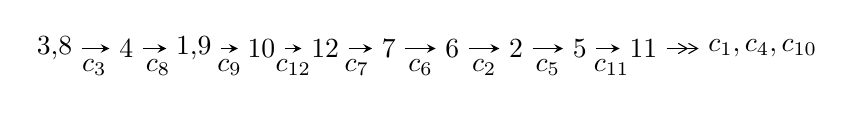
\begin{tikzpicture}[x=23pt, y=7pt]
	% node
	\node (A0) at (-1/8, 0) {3,8};
	\node (A1) at (1, 0) {4};
	\node (A2) at (33/16, 0) {1,9};
	\node (A3) at (25/8, 0) {10};
	\node (A4) at (33/8, 0) {12};
	\node (A5) at (41/8, 0) {7};
	\node (A6) at (49/8, 0) {6};
	\node (A7) at (57/8, 0) {2};
	\node (A8) at (65/8, 0) {5};
	\node (A9) at (73/8, 0) {11};
	\node (C1) at (1/2, -1) {$c_{3}$};
	\node (C2) at (3/2, -1) {$c_{8}$};
	\node (C3) at (21/8, -1) {$c_{9}$};
	\node (C4) at (29/8, -1) {$c_{12}$};
	\node (C5) at (37/8, -1) {$c_{7}$};
	\node (C6) at (45/8, -1) {$c_{6}$};
	\node (C7) at (53/8, -1) {$c_{2}$};
	\node (C8) at (61/8, -1) {$c_{5}$};
	\node (C9) at (69/8, -1) {$c_{11}$};
	\node (A10) at (11, 0) {$c_{1},c_{4},c_{10}$};

	% edge
	\draw[->,>=stealth]	
	(A0) edge (A1) (A1) edge (A2) (A2) edge (A3) (A3) edge (A4) (A4) edge (A5) (A5) edge (A6) (A6) edge (A7) (A7) edge (A8) (A8) edge (A9) ;
	\draw[->>,>={angle 60}]	
	(A9) edge (A10);
\end{tikzpicture} \\ 

\end{tabular} \\

\footnotetext{
The image of knot diagram is generated by the software ``\textbf{Draw programme}" developed by Andrew Bartholomew(\url{http://www.layer8.co.uk/maths/draw/index.htm\#Running-draw}), where we modified some parts for our purpose(\url{https://github.com/CATsTAILs/LinksPainter}).
}\phantom \\ \newline 
\centering \textbf{Ideals for irreducible components\footnotemark of $X_{\text{par}}$} 
 
\begin{align*}
I^u_{1}&=\langle 
465502349422 u^{14}-79727868434 u^{13}+\cdots+599549983265 b+123387962359,\\
\phantom{I^u_{1}}&\phantom{= \langle  }851737214407 u^{14}-547553851564 u^{13}+\cdots+599549983265 a-2100202102861,\\
\phantom{I^u_{1}}&\phantom{= \langle  }u^{15}-14 u^{13}-4 u^{12}+107 u^{11}+26 u^{10}-207 u^9-86 u^8+119 u^7-16 u^6+74 u^5+44 u^4+3 u^3+7 u^2-1\rangle \\
I^u_{2}&=\langle 
-8 u^9+12 u^8-14 u^7+7 u^6+8 u^5-36 u^4+17 u^3-29 u^2+25 b-13 u+34,\\
\phantom{I^u_{2}}&\phantom{= \langle  }-63 u^9+32 u^8-54 u^7-23 u^6+163 u^5-171 u^4+112 u^3-19 u^2+25 a-293 u+149,\\
\phantom{I^u_{2}}&\phantom{= \langle  }u^{10}- u^9+u^8-3 u^6+4 u^5-3 u^4+u^3+5 u^2-5 u+1\rangle \\
\\
\end{align*}
\raggedright * 2 irreducible components of $\dim_{\mathbb{C}}=0$, with total 25 representations.\\
\footnotetext{All coefficients of polynomials are rational numbers. But the coefficients are sometimes approximated in decimal forms when there is not enough margin.}
\newpage
\renewcommand{\arraystretch}{1}
\centering \section*{I. $I^u_{1}= \langle 4.66\times10^{11} u^{14}-7.97\times10^{10} u^{13}+\cdots+6.00\times10^{11} b+1.23\times10^{11},\;8.52\times10^{11} u^{14}-5.48\times10^{11} u^{13}+\cdots+6.00\times10^{11} a-2.10\times10^{12},\;u^{15}-14 u^{13}+\cdots+7 u^2-1 \rangle$}
\flushleft \textbf{(i) Arc colorings}\\
\begin{tabular}{m{7pt} m{180pt} m{7pt} m{180pt} }
\flushright $a_{3}=$&$\begin{pmatrix}1\\0\end{pmatrix}$ \\
\flushright $a_{8}=$&$\begin{pmatrix}0\\u\end{pmatrix}$ \\
\flushright $a_{4}=$&$\begin{pmatrix}1\\- u^2\end{pmatrix}$ \\
\flushright $a_{1}=$&$\begin{pmatrix}-1.42063 u^{14}+0.913275 u^{13}+\cdots+1.01409 u+3.50296\\-0.776420 u^{14}+0.132980 u^{13}+\cdots-1.17993 u-0.205801\end{pmatrix}$ \\
\flushright $a_{9}=$&$\begin{pmatrix}u\\u\end{pmatrix}$ \\
\flushright $a_{10}=$&$\begin{pmatrix}-1.49471 u^{14}-0.580434 u^{13}+\cdots-14.9172 u+0.00184502\\0.320071 u^{14}-0.134431 u^{13}+\cdots+2.49471 u+0.580434\end{pmatrix}$ \\
\flushright $a_{12}=$&$\begin{pmatrix}-1.42063 u^{14}+0.913275 u^{13}+\cdots+1.01409 u+3.50296\\-0.792950 u^{14}+0.229300 u^{13}+\cdots+0.240700 u-1.11908\end{pmatrix}$ \\
\flushright $a_{7}=$&$\begin{pmatrix}0.718288 u^{14}+0.713414 u^{13}+\cdots+13.7373 u-0.207646\\-0.977277 u^{14}+0.474429 u^{13}+\cdots-1.89822 u-0.919215\end{pmatrix}$ \\
\flushright $a_{6}=$&$\begin{pmatrix}-0.468813 u^{14}-0.416564 u^{13}+\cdots-3.44802 u-5.40828\\-0.702958 u^{14}+0.430796 u^{13}+\cdots-1.35532 u+0.991058\end{pmatrix}$ \\
\flushright $a_{2}=$&$\begin{pmatrix}-0.644208 u^{14}+0.780295 u^{13}+\cdots+2.19402 u+3.70877\\-0.776420 u^{14}+0.132980 u^{13}+\cdots-1.17993 u-0.205801\end{pmatrix}$ \\
\flushright $a_{5}=$&$\begin{pmatrix}-0.580434 u^{14}-0.320071 u^{13}+\cdots+0.00184502 u-2.49471\\-0.134431 u^{14}-0.0198011 u^{13}+\cdots+0.580434 u+0.320071\end{pmatrix}$ \\
\flushright $a_{11}=$&$\begin{pmatrix}-1.49471 u^{14}-0.580434 u^{13}+\cdots-13.9172 u+0.00184502\\0.320071 u^{14}-0.134431 u^{13}+\cdots+2.49471 u+0.580434\end{pmatrix}$\\&\end{tabular}
\flushleft \textbf{(ii) Obstruction class $= -1$}\\~\\
\flushleft \textbf{(iii) Cusp Shapes $= \frac{2849816670076}{599549983265} u^{14}-\frac{2328924086222}{599549983265} u^{13}+\cdots-\frac{4273891768151}{599549983265} u-\frac{9195265038463}{599549983265}$}\\~\\
\newpage\renewcommand{\arraystretch}{1}
\flushleft \textbf{(iv) u-Polynomials at the component}\newline \\
\begin{tabular}{m{50pt}|m{274pt}}
Crossings & \hspace{64pt}u-Polynomials at each crossing \\
\hline $$\begin{aligned}c_{1}\end{aligned}$$&$\begin{aligned}
&u^{15}+3 u^{14}+\cdots+9 u+1
\end{aligned}$\\
\hline $$\begin{aligned}c_{2},c_{5}\end{aligned}$$&$\begin{aligned}
&u^{15}+3 u^{14}+\cdots+u+1
\end{aligned}$\\
\hline $$\begin{aligned}c_{3},c_{4},c_{8}\\c_{10}\end{aligned}$$&$\begin{aligned}
&u^{15}-14 u^{13}+\cdots+7 u^2-1
\end{aligned}$\\
\hline $$\begin{aligned}c_{6},c_{9}\end{aligned}$$&$\begin{aligned}
&u^{15}+u^{14}+\cdots-17 u+1
\end{aligned}$\\
\hline $$\begin{aligned}c_{7},c_{11},c_{12}\end{aligned}$$&$\begin{aligned}
&u^{15}-14 u^{14}+\cdots-96 u+32
\end{aligned}$\\
\hline
\end{tabular}\\~\\
\newpage\renewcommand{\arraystretch}{1}
\flushleft \textbf{(v) Riley Polynomials at the component}\newline \\
\begin{tabular}{m{50pt}|m{274pt}}
Crossings & \hspace{64pt}Riley Polynomials at each crossing \\
\hline $$\begin{aligned}c_{1}\end{aligned}$$&$\begin{aligned}
&y^{15}+21 y^{14}+\cdots+9 y-1
\end{aligned}$\\
\hline $$\begin{aligned}c_{2},c_{5}\end{aligned}$$&$\begin{aligned}
&y^{15}-3 y^{14}+\cdots+9 y-1
\end{aligned}$\\
\hline $$\begin{aligned}c_{3},c_{4},c_{8}\\c_{10}\end{aligned}$$&$\begin{aligned}
&y^{15}-28 y^{14}+\cdots+14 y-1
\end{aligned}$\\
\hline $$\begin{aligned}c_{6},c_{9}\end{aligned}$$&$\begin{aligned}
&y^{15}+39 y^{14}+\cdots+295 y-1
\end{aligned}$\\
\hline $$\begin{aligned}c_{7},c_{11},c_{12}\end{aligned}$$&$\begin{aligned}
&y^{15}-10 y^{14}+\cdots+4608 y-1024
\end{aligned}$\\
\hline
\end{tabular}\\~\\
\newpage\flushleft \textbf{(vi) Complex Volumes and Cusp Shapes}
$$\begin{array}{c|c|c}  
\text{Solutions to }I^u_{1}& \I (\text{vol} + \sqrt{-1}CS) & \text{Cusp shape}\\
 \hline 
\begin{aligned}
u &= \phantom{-}1.286970 + 0.003568 I \\
a &= \phantom{-}0.589686 - 0.744025 I \\
b &= \phantom{-}0.319963 - 1.267150 I\end{aligned}
 & \phantom{-}4.37389 + 0.30095 I & -3.29649 - 1.17688 I \\ \hline\begin{aligned}
u &= \phantom{-}1.286970 - 0.003568 I \\
a &= \phantom{-}0.589686 + 0.744025 I \\
b &= \phantom{-}0.319963 + 1.267150 I\end{aligned}
 & \phantom{-}4.37389 - 0.30095 I & -3.29649 + 1.17688 I \\ \hline\begin{aligned}
u &= -1.220550 + 0.546816 I \\
a &= -0.491530 - 0.908635 I \\
b &= -0.47712 - 1.50755 I\end{aligned}
 & \phantom{-}3.32606 - 6.34337 I & -6.36496 + 6.14476 I \\ \hline\begin{aligned}
u &= -1.220550 - 0.546816 I \\
a &= -0.491530 + 0.908635 I \\
b &= -0.47712 + 1.50755 I\end{aligned}
 & \phantom{-}3.32606 + 6.34337 I & -6.36496 - 6.14476 I \\ \hline\begin{aligned}
u &= \phantom{-}0.100194 + 0.555594 I \\
a &= \phantom{-}0.55980 - 2.69568 I \\
b &= -0.253685 - 0.984505 I\end{aligned}
 & -6.84743 - 2.37164 I & -5.86485 + 4.49258 I \\ \hline\begin{aligned}
u &= \phantom{-}0.100194 - 0.555594 I \\
a &= \phantom{-}0.55980 + 2.69568 I \\
b &= -0.253685 + 0.984505 I\end{aligned}
 & -6.84743 + 2.37164 I & -5.86485 - 4.49258 I \\ \hline\begin{aligned}
u &= \phantom{-}0.053551 + 0.530205 I \\
a &= \phantom{-}0.648734 + 0.711885 I \\
b &= -0.067055 + 0.375797 I\end{aligned}
 & -0.327240 + 1.083790 I & -4.63730 - 6.18366 I \\ \hline\begin{aligned}
u &= \phantom{-}0.053551 - 0.530205 I \\
a &= \phantom{-}0.648734 - 0.711885 I \\
b &= -0.067055 - 0.375797 I\end{aligned}
 & -0.327240 - 1.083790 I & -4.63730 + 6.18366 I \\ \hline\begin{aligned}
u &= -0.453145\phantom{ +0.000000I} \\
a &= -1.45303\phantom{ +0.000000I} \\
b &= -1.32667\phantom{ +0.000000I}\end{aligned}
 & -2.54518\phantom{ +0.000000I} & \phantom{-}9.96520\phantom{ +0.000000I} \\ \hline\begin{aligned}
u &= -0.384303\phantom{ +0.000000I} \\
a &= \phantom{-}1.94891\phantom{ +0.000000I} \\
b &= -0.219731\phantom{ +0.000000I}\end{aligned}
 & -1.51666\phantom{ +0.000000I} & -4.64930\phantom{ +0.000000I}\\
 \hline 
 \end{array}$$\newpage$$\begin{array}{c|c|c}  
\text{Solutions to }I^u_{1}& \I (\text{vol} + \sqrt{-1}CS) & \text{Cusp shape}\\
 \hline 
\begin{aligned}
u &= \phantom{-}0.278558\phantom{ +0.000000I} \\
a &= \phantom{-}5.85314\phantom{ +0.000000I} \\
b &= -0.441847\phantom{ +0.000000I}\end{aligned}
 & -9.80649\phantom{ +0.000000I} & -23.6470\phantom{ +0.000000I} \\ \hline\begin{aligned}
u &= \phantom{-}2.72441 + 1.12795 I \\
a &= \phantom{-}0.289084 - 0.671320 I \\
b &= \phantom{-}0.08254 - 1.84271 I\end{aligned}
 & \phantom{-}16.0556 + 2.2374 I & -4.43024 + 0. I\phantom{ +0.000000I} \\ \hline\begin{aligned}
u &= \phantom{-}2.72441 - 1.12795 I \\
a &= \phantom{-}0.289084 + 0.671320 I \\
b &= \phantom{-}0.08254 + 1.84271 I\end{aligned}
 & \phantom{-}16.0556 - 2.2374 I & -4.43024 + 0. I\phantom{ +0.000000I} \\ \hline\begin{aligned}
u &= -2.66513 + 1.31852 I \\
a &= -0.270282 - 0.679151 I \\
b &= -0.11052 - 1.88022 I\end{aligned}
 & \phantom{-}15.8498 - 9.2839 I & -4.74065 + 4.04193 I \\ \hline\begin{aligned}
u &= -2.66513 - 1.31852 I \\
a &= -0.270282 + 0.679151 I \\
b &= -0.11052 + 1.88022 I\end{aligned}
 & \phantom{-}15.8498 + 9.2839 I & -4.74065 - 4.04193 I\\
 \hline 
 \end{array}$$\newpage\newpage\renewcommand{\arraystretch}{1}
\centering \section*{II. $I^u_{2}= \langle -8 u^9+12 u^8+\cdots+25 b+34,\;-63 u^9+32 u^8+\cdots+25 a+149,\;u^{10}- u^9+\cdots-5 u+1 \rangle$}
\flushleft \textbf{(i) Arc colorings}\\
\begin{tabular}{m{7pt} m{180pt} m{7pt} m{180pt} }
\flushright $a_{3}=$&$\begin{pmatrix}1\\0\end{pmatrix}$ \\
\flushright $a_{8}=$&$\begin{pmatrix}0\\u\end{pmatrix}$ \\
\flushright $a_{4}=$&$\begin{pmatrix}1\\- u^2\end{pmatrix}$ \\
\flushright $a_{1}=$&$\begin{pmatrix}2.52000 u^{9}-1.28000 u^{8}+\cdots+11.7200 u-5.96000\\0.320000 u^{9}-0.480000 u^{8}+\cdots+0.520000 u-1.36000\end{pmatrix}$ \\
\flushright $a_{9}=$&$\begin{pmatrix}u\\u\end{pmatrix}$ \\
\flushright $a_{10}=$&$\begin{pmatrix}-1.52000 u^{9}+0.280000 u^{8}+\cdots-6.72000 u+0.960000\\0.880000 u^{9}-0.320000 u^{8}+\cdots+3.68000 u-1.24000\end{pmatrix}$ \\
\flushright $a_{12}=$&$\begin{pmatrix}2.52000 u^{9}-1.28000 u^{8}+\cdots+11.7200 u-5.96000\\-0.560000 u^{9}-0.160000 u^{8}+\cdots-3.16000 u-0.120000\end{pmatrix}$ \\
\flushright $a_{7}=$&$\begin{pmatrix}\frac{6}{5} u^9+\frac{1}{5} u^8+\cdots+\frac{31}{5} u+\frac{2}{5}\\-1.12000 u^{9}+0.680000 u^{8}+\cdots-6.32000 u+2.76000\end{pmatrix}$ \\
\flushright $a_{6}=$&$\begin{pmatrix}-2.52000 u^{9}+1.28000 u^{8}+\cdots-12.7200 u+5.96000\\-0.240000 u^{9}+0.360000 u^{8}+\cdots-1.64000 u+1.52000\end{pmatrix}$ \\
\flushright $a_{2}=$&$\begin{pmatrix}\frac{11}{5} u^9-\frac{4}{5} u^8+\cdots+\frac{56}{5} u-\frac{23}{5}\\0.320000 u^{9}-0.480000 u^{8}+\cdots+0.520000 u-1.36000\end{pmatrix}$ \\
\flushright $a_{5}=$&$\begin{pmatrix}-1.24000 u^{9}+0.360000 u^{8}+\cdots-6.64000 u+2.52000\\0.560000 u^{9}+0.160000 u^{8}+\cdots+3.16000 u-0.880000\end{pmatrix}$ \\
\flushright $a_{11}=$&$\begin{pmatrix}-1.52000 u^{9}+0.280000 u^{8}+\cdots-7.72000 u+0.960000\\0.880000 u^{9}-0.320000 u^{8}+\cdots+3.68000 u-1.24000\end{pmatrix}$\\&\end{tabular}
\flushleft \textbf{(ii) Obstruction class $= 1$}\\~\\
\flushleft \textbf{(iii) Cusp Shapes $= \frac{303}{25} u^9-\frac{167}{25} u^8+\frac{249}{25} u^7+\frac{88}{25} u^6-\frac{878}{25} u^5+\frac{826}{25} u^4-\frac{622}{25} u^3+\frac{114}{25} u^2+\frac{1558}{25} u-\frac{944}{25}$}\\~\\
\newpage\renewcommand{\arraystretch}{1}
\flushleft \textbf{(iv) u-Polynomials at the component}\newline \\
\begin{tabular}{m{50pt}|m{274pt}}
Crossings & \hspace{64pt}u-Polynomials at each crossing \\
\hline $$\begin{aligned}c_{1}\end{aligned}$$&$\begin{aligned}
&u^{10}-2 u^9+9 u^8-15 u^7+28 u^6-38 u^5+35 u^4-31 u^3+15 u^2-6 u+1
\end{aligned}$\\
\hline $$\begin{aligned}c_{2}\end{aligned}$$&$\begin{aligned}
&u^{10}+2 u^9+u^8-3 u^7-2 u^6+2 u^5+3 u^4-3 u^3-3 u^2+1
\end{aligned}$\\
\hline $$\begin{aligned}c_{3},c_{10}\end{aligned}$$&$\begin{aligned}
&u^{10}- u^9+u^8-3 u^6+4 u^5-3 u^4+u^3+5 u^2-5 u+1
\end{aligned}$\\
\hline $$\begin{aligned}c_{4},c_{8}\end{aligned}$$&$\begin{aligned}
&u^{10}+u^9+u^8-3 u^6-4 u^5-3 u^4- u^3+5 u^2+5 u+1
\end{aligned}$\\
\hline $$\begin{aligned}c_{5}\end{aligned}$$&$\begin{aligned}
&u^{10}-2 u^9+u^8+3 u^7-2 u^6-2 u^5+3 u^4+3 u^3-3 u^2+1
\end{aligned}$\\
\hline $$\begin{aligned}c_{6},c_{9}\end{aligned}$$&$\begin{aligned}
&u^{10}+3 u^7-5 u^6+2 u^5-3 u^4-2 u^2+8 u-3
\end{aligned}$\\
\hline $$\begin{aligned}c_{7}\end{aligned}$$&$\begin{aligned}
&u^{10}-5 u^8+3 u^7+10 u^6-9 u^5-7 u^4+9 u^3+u^2- u-1
\end{aligned}$\\
\hline $$\begin{aligned}c_{11},c_{12}\end{aligned}$$&$\begin{aligned}
&u^{10}-5 u^8-3 u^7+10 u^6+9 u^5-7 u^4-9 u^3+u^2+u-1
\end{aligned}$\\
\hline
\end{tabular}\\~\\
\newpage\renewcommand{\arraystretch}{1}
\flushleft \textbf{(v) Riley Polynomials at the component}\newline \\
\begin{tabular}{m{50pt}|m{274pt}}
Crossings & \hspace{64pt}Riley Polynomials at each crossing \\
\hline $$\begin{aligned}c_{1}\end{aligned}$$&$\begin{aligned}
&y^{10}+14 y^9+\cdots-6 y+1
\end{aligned}$\\
\hline $$\begin{aligned}c_{2},c_{5}\end{aligned}$$&$\begin{aligned}
&y^{10}-2 y^9+9 y^8-15 y^7+28 y^6-38 y^5+35 y^4-31 y^3+15 y^2-6 y+1
\end{aligned}$\\
\hline $$\begin{aligned}c_{3},c_{4},c_{8}\\c_{10}\end{aligned}$$&$\begin{aligned}
&y^{10}+y^9-5 y^8-4 y^7+15 y^6+4 y^5-27 y^4+3 y^3+29 y^2-15 y+1
\end{aligned}$\\
\hline $$\begin{aligned}c_{6},c_{9}\end{aligned}$$&$\begin{aligned}
&y^{10}-10 y^8-15 y^7+9 y^6+20 y^5-19 y^4+10 y^3+22 y^2-52 y+9
\end{aligned}$\\
\hline $$\begin{aligned}c_{7},c_{11},c_{12}\end{aligned}$$&$\begin{aligned}
&y^{10}-10 y^9+\cdots-3 y+1
\end{aligned}$\\
\hline
\end{tabular}\\~\\
\newpage\flushleft \textbf{(vi) Complex Volumes and Cusp Shapes}
$$\begin{array}{c|c|c}  
\text{Solutions to }I^u_{2}& \I (\text{vol} + \sqrt{-1}CS) & \text{Cusp shape}\\
 \hline 
\begin{aligned}
u &= \phantom{-}1.047150 + 0.419466 I \\
a &= -0.745457 + 0.844492 I \\
b &= -0.28578 + 1.89933 I\end{aligned}
 & \phantom{-}5.01632 + 5.84673 I & -1.85887 - 5.25090 I \\ \hline\begin{aligned}
u &= \phantom{-}1.047150 - 0.419466 I \\
a &= -0.745457 - 0.844492 I \\
b &= -0.28578 - 1.89933 I\end{aligned}
 & \phantom{-}5.01632 - 5.84673 I & -1.85887 + 5.25090 I \\ \hline\begin{aligned}
u &= -1.154050 + 0.132803 I \\
a &= \phantom{-}0.775839 + 0.664119 I \\
b &= \phantom{-}0.24316 + 1.73359 I\end{aligned}
 & \phantom{-}5.60821 + 1.13028 I & -1.128175 - 0.572443 I \\ \hline\begin{aligned}
u &= -1.154050 - 0.132803 I \\
a &= \phantom{-}0.775839 - 0.664119 I \\
b &= \phantom{-}0.24316 - 1.73359 I\end{aligned}
 & \phantom{-}5.60821 - 1.13028 I & -1.128175 + 0.572443 I \\ \hline\begin{aligned}
u &= \phantom{-}0.734349\phantom{ +0.000000I} \\
a &= \phantom{-}2.32032\phantom{ +0.000000I} \\
b &= -0.271586\phantom{ +0.000000I}\end{aligned}
 & -9.51751\phantom{ +0.000000I} & \phantom{-}4.60600\phantom{ +0.000000I} \\ \hline\begin{aligned}
u &= \phantom{-}0.328497 + 1.235550 I \\
a &= \phantom{-}0.448610 - 0.982537 I \\
b &= -0.188603 - 0.504750 I\end{aligned}
 & -7.98285 - 1.51634 I & -9.37010 + 3.27052 I \\ \hline\begin{aligned}
u &= \phantom{-}0.328497 - 1.235550 I \\
a &= \phantom{-}0.448610 + 0.982537 I \\
b &= -0.188603 + 0.504750 I\end{aligned}
 & -7.98285 + 1.51634 I & -9.37010 - 3.27052 I \\ \hline\begin{aligned}
u &= -0.228999 + 1.295180 I \\
a &= \phantom{-}0.201014 - 0.252463 I \\
b &= -0.068161 - 0.994177 I\end{aligned}
 & -3.05365 - 2.41009 I & -4.28312 + 3.73455 I \\ \hline\begin{aligned}
u &= -0.228999 - 1.295180 I \\
a &= \phantom{-}0.201014 + 0.252463 I \\
b &= -0.068161 + 0.994177 I\end{aligned}
 & -3.05365 + 2.41009 I & -4.28312 - 3.73455 I \\ \hline\begin{aligned}
u &= \phantom{-}0.280460\phantom{ +0.000000I} \\
a &= -2.68033\phantom{ +0.000000I} \\
b &= -1.12964\phantom{ +0.000000I}\end{aligned}
 & -2.81801\phantom{ +0.000000I} & -20.3250\phantom{ +0.000000I}\\
 \hline 
 \end{array}$$\newpage
\newpage\renewcommand{\arraystretch}{1}
\centering \section*{ III. u-Polynomials}
\begin{tabular}{m{50pt}|m{274pt}}
Crossings & \hspace{64pt}u-Polynomials at each crossing \\
\hline $$\begin{aligned}c_{1}\end{aligned}$$&$\begin{aligned}
&(u^{10}-2 u^9+9 u^8-15 u^7+28 u^6-38 u^5+35 u^4-31 u^3+15 u^2-6 u+1)\\
&\cdot(u^{15}+3 u^{14}+\cdots+9 u+1)
\end{aligned}$\\
\hline $$\begin{aligned}c_{2}\end{aligned}$$&$\begin{aligned}
&(u^{10}+2 u^9+u^8-3 u^7-2 u^6+2 u^5+3 u^4-3 u^3-3 u^2+1)\\
&\cdot(u^{15}+3 u^{14}+\cdots+u+1)
\end{aligned}$\\
\hline $$\begin{aligned}c_{3},c_{10}\end{aligned}$$&$\begin{aligned}
&(u^{10}- u^9+u^8-3 u^6+4 u^5-3 u^4+u^3+5 u^2-5 u+1)\\
&\cdot(u^{15}-14 u^{13}+\cdots+7 u^2-1)
\end{aligned}$\\
\hline $$\begin{aligned}c_{4},c_{8}\end{aligned}$$&$\begin{aligned}
&(u^{10}+u^9+u^8-3 u^6-4 u^5-3 u^4- u^3+5 u^2+5 u+1)\\
&\cdot(u^{15}-14 u^{13}+\cdots+7 u^2-1)
\end{aligned}$\\
\hline $$\begin{aligned}c_{5}\end{aligned}$$&$\begin{aligned}
&(u^{10}-2 u^9+u^8+3 u^7-2 u^6-2 u^5+3 u^4+3 u^3-3 u^2+1)\\
&\cdot(u^{15}+3 u^{14}+\cdots+u+1)
\end{aligned}$\\
\hline $$\begin{aligned}c_{6},c_{9}\end{aligned}$$&$\begin{aligned}
&(u^{10}+3 u^7+\cdots+8 u-3)(u^{15}+u^{14}+\cdots-17 u+1)
\end{aligned}$\\
\hline $$\begin{aligned}c_{7}\end{aligned}$$&$\begin{aligned}
&(u^{10}-5 u^8+3 u^7+10 u^6-9 u^5-7 u^4+9 u^3+u^2- u-1)\\
&\cdot(u^{15}-14 u^{14}+\cdots-96 u+32)
\end{aligned}$\\
\hline $$\begin{aligned}c_{11},c_{12}\end{aligned}$$&$\begin{aligned}
&(u^{10}-5 u^8-3 u^7+10 u^6+9 u^5-7 u^4-9 u^3+u^2+u-1)\\
&\cdot(u^{15}-14 u^{14}+\cdots-96 u+32)
\end{aligned}$\\
\hline
\end{tabular}\newpage\renewcommand{\arraystretch}{1}
\centering \section*{ IV. Riley Polynomials}
\begin{tabular}{m{50pt}|m{274pt}}
Crossings & \hspace{64pt}Riley Polynomials at each crossing \\
\hline $$\begin{aligned}c_{1}\end{aligned}$$&$\begin{aligned}
&(y^{10}+14 y^9+\cdots-6 y+1)(y^{15}+21 y^{14}+\cdots+9 y-1)
\end{aligned}$\\
\hline $$\begin{aligned}c_{2},c_{5}\end{aligned}$$&$\begin{aligned}
&(y^{10}-2 y^9+9 y^8-15 y^7+28 y^6-38 y^5+35 y^4-31 y^3+15 y^2-6 y+1)\\
&\cdot(y^{15}-3 y^{14}+\cdots+9 y-1)
\end{aligned}$\\
\hline $$\begin{aligned}c_{3},c_{4},c_{8}\\c_{10}\end{aligned}$$&$\begin{aligned}
&(y^{10}+y^9-5 y^8-4 y^7+15 y^6+4 y^5-27 y^4+3 y^3+29 y^2-15 y+1)\\
&\cdot(y^{15}-28 y^{14}+\cdots+14 y-1)
\end{aligned}$\\
\hline $$\begin{aligned}c_{6},c_{9}\end{aligned}$$&$\begin{aligned}
&(y^{10}-10 y^8-15 y^7+9 y^6+20 y^5-19 y^4+10 y^3+22 y^2-52 y+9)\\
&\cdot(y^{15}+39 y^{14}+\cdots+295 y-1)
\end{aligned}$\\
\hline $$\begin{aligned}c_{7},c_{11},c_{12}\end{aligned}$$&$\begin{aligned}
&(y^{10}-10 y^9+\cdots-3 y+1)(y^{15}-10 y^{14}+\cdots+4608 y-1024)
\end{aligned}$\\
\hline
\end{tabular}
\vskip 2pc
\end{document}